\documentclass{homework}
\usepackage{cancel}
\usepackage{amsthm}
\usepackage{cleveref}
\usepackage{upgreek}
\usepackage[framed]{mcode}
\usepackage{mathrsfs}
\usepackage{tikz,pgf}
\usepackage{units}
\usetikzlibrary{matrix}
\usetikzlibrary{arrows}
\newtheorem{lemma}{Lemma}

\title{Kevin Joyce}
\course{Math 512 - Integral Equations - Final}
\author{Kevin Joyce}
\docdate{\today}
\begin{document} 
\newcommand{\figref}[1]{\figurename~\ref{#1}}
\renewcommand{\bar}{\overline}
\renewcommand{\hat}{\widehat}
\renewcommand{\SS}{\mathcal S}
\renewcommand{\NN}{\mathcal N}
\newcommand{\DD}{\mathcal D}
\newcommand{\eps}{\varepsilon}
\newcommand{\del}{\partial}

\problem{ Is the sequence $y_n = x^n$ compact }

\subproblem{ in $C[0,1]$? }
\begin{solution}
  This sequence is not compact in this space.  For $\{y_n\}$ we have
  \begin{align*}
    \|y_n - y_{2n}\|_{C[0,1]} 
    = \sup_{x\in[0,1]} | x^n - x^{2n} |
    \ge \left.\Big(| x^n - x^{2n} | \Big)\right|_{x=\left(\frac 12\right)^{1/n}} = \frac 14
  \end{align*}
  \begin{center}
  % The following codes were adapted from automatically generated code from the program Geogebra
  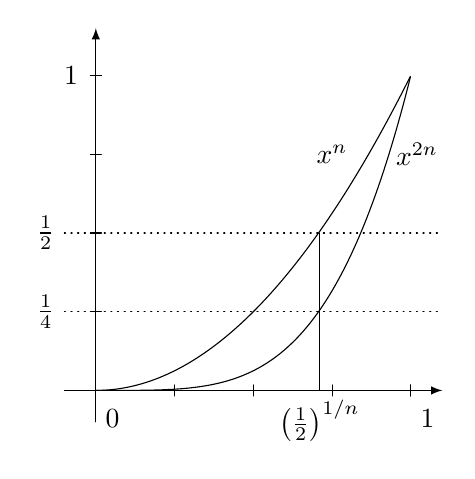
\begin{tikzpicture}[line cap=round,line join=round,>=latex,x=4cm,y=4cm]
  % Draw axes
  \draw[->,color=black] (-0.1,0) -- (1.1,0);
  \foreach \x in {,0.25,0.5,0.75,1}
    \draw[shift={(\x,0)},color=black] (0pt,2pt) -- (0pt,-2pt);

  \draw[->,color=black] (0,-0.1) -- (0,1.15);
  \foreach \y in {,0.25,0.5,0.75,1}
    \draw[shift={(0,\y)},color=black] (2pt,0pt) -- (-2pt,0pt);

  % Labels
  \draw[color=black] (0pt,-10pt) node[right] {$0$};
  \draw[color=black] (1,-10pt) node[right]   {$1$};
  \draw[color=black] (-15pt,1) node[right]   {$1$};
  \node  at (.75,.75){$x^n$};
  \node  at (1.02,.75){$x^{2n}$};

  % Draw curves
  \draw[smooth,samples=100,domain=0.0:1.0] plot(\x,{(\x)^2});
  \draw[smooth,samples=100,domain=0.0:1.0] plot(\x,{(\x)^4});

  % Dotted lines
  \draw [dotted] (-.1,.5) node[left] {$\frac 12$} -- (1.1,.5);
  \draw [dotted] (-.1,.25) node[left] {$\frac 14$} -- (1.1,.25);

  % Vertical line
  \draw (0.71,0.5)-- (0.71,0) node[below] {$\left(\frac 12\right)^{1/n}$};
  \end{tikzpicture}
  \end{center}

  Hence $\{y_n\}$ has no points of accumulation, and thus cannot be compact.
\end{solution}

\subproblem{ in $h[0,1]$? }

\begin{solution}
  The sequence is compact in this space.  In fact, it is Cauchy, since
  \begin{align*}
    \|y_n - y_m\|_{h[0,1]}^2 
    &= \|y_{n}\|_{h[0,1]}^2 - 2\Big(y_n,y_m\Big) + \|y_m\|_{h[0,1]}^2 \\
    &= \int_0^1 x^{2n}\,dx - 2\int_0^1x^{n+m}\,dx + \int_0^2 x^{2m}\,dx \\
    &= \frac 1{2n+1} - 2\frac 1{n+m+1} + \frac 1{2m+1} \to 0\quad\text{ as }m,n\to \infty.
  \end{align*}
  So \emph{every} subsequence has a point of accumulation.
\end{solution}
\newpage
\problem{ Find characteristic values and eigenfunctions: 
$$
  y(x) = \lambda\int_{-1}^1 (xs +x^2s^2)\,y(s)\,ds
$$
}

\begin{solution}
  Let $f_1(x) = x$ and $f_2(x) = x^2$.  Note that these are linearly independent. An eigenvector $y$ satisfies
\begin{align*}
    y &= \lambda \left(x\int_{-1}^1 sy(s) \,ds + x^2 \int_{-1}^1 s^2y(s)\,ds\right) = \lambda \left\{ \Big(f_1,y\Big)f_1(x) + \Big(f_2,y\Big)f_2(x)\right\}.\\
\end{align*}

Taking inner products on both sides with both $f_1$ and $f_2$, we arrive at the linear system
\renewcommand{\arraystretch}{2}
$$
  \begin{bmatrix}
    \Big(f_1,y\Big)\\
    \Big(f_2,y\Big)
  \end{bmatrix}
   = \lambda \begin{bmatrix}
  \Big(f_1,f_1\Big) & \Big(f_1,f_2\Big) \\
  \Big(f_2,f_1\Big) & \Big(f_2,f_2\Big) \\
  \end{bmatrix} 
  \begin{bmatrix}
    \Big(f_1,y\Big)\\
    \Big(f_2,y\Big)
  \end{bmatrix}
  \iff
  Y = \lambda M Y.
$$
The entries of $M$ are given by
\begin{align*}
\begin{array}{rl}
  (f_1,f_1)	      &= \ds{\int_{-1}^1 x^2\,dx = \frac 23},\\
(f_2,f_1) = (f_1,f_2) &=\ds{ \int_{-1}^1 x^3\,dx = 0},\\
  (f_2,f_2)	      &=\ds{ \int_{-1}^1 x^4\,dx = \frac 25.}
\end{array}
\quad \text{So }
M = \begin{bmatrix}
\ds{\frac 23} & 0\\
0        & \ds{\frac 25}\\
\end{bmatrix}.
\end{align*}
Hence, the characteristic values satisfy
$$
\renewcommand{\arraystretch}{2}
  0=\left|\lambda M - I\right| 
  = \left|\begin{array}{ccc}
    \frac 23\lambda - 1 & 0 \\
    0 &  \frac 25 \lambda -1\\
  \end{array}
  \right|
  \iff \lambda_1 = \frac 32\text{ or }\lambda_2=\frac 52.
$$
Since $M$ is diagonal, the corresponding eigenvectors of coeffcients are given by $\binom {c_1}0$ and $\binom 0{c_2}$, and, thus $y_1 = \frac 32 c_1 x$ and $y_2 = \frac 52 c_2 x^2$. 

\end{solution}
\newpage

\problem{ Construct the Neumann series for the Volterra equation of the second kind 
$$
  y(x) = \lambda \int_0^x s\,y(s)\,ds + 1
$$
and find the solution.
}

\begin{solution}
  Let $A$ be the integral operator $\int_0^x \cdot \,s ds$ and $f \equiv 1$. It can be shown that the map $y\mapsto \lambda Ay + f$ is a contraction operator whose fixed point is the solution and is given by repeated composition to an arbitrary function $y_0$.  Successive applications of this map to $y_0 = 0$ yields the Neumann series
  \begin{equation}
    y_{n+1} = f + \lambda Af + \lambda^2 A^2 f + \dots + \lambda^n A^n f. \label{neumann}
  \end{equation}
  Note that
  \begin{align}
    A f = \int_0^x s ds &= \frac {x^2}2, \nonumber\\
    A^2 f = \int_0^x \frac {s^2}2 s ds &= \frac {x^4}{2\cdot4}, \nonumber\\
    A^3 f = \int_0^x \frac {s^4}{2\cdot4} s ds &= \frac {x^6}{2\cdot4\cdot6}, \nonumber\\
    \vdots\nonumber\\
    A^n f = \int_0^x \frac {s^{2n} }{2^nn!} sds &= \frac {x^{2n+2}}{2^{n+1}(n+1)!}. \label{kern1}
  \end{align}
  So,% for $\lambda \not=0$ and $x\not=0$,
  $$
    y = \lim_{n\to\infty} y_n = \sum_{k=0}^\infty \frac{\left( \frac \lambda 2 x^2 \right)^k}{k!} = e^{\frac\lambda 2x^2}.
  $$

  We can easily verify that $y$ is a solution,
  $$
    \lambda \int_0^x s e^{\frac\lambda2 s^2} + 1 = \lambda \int_0^{\frac \lambda2 x^2} e^u\,du+1 = e^{\frac\lambda2 x^2} -1 + 1=e^{\frac\lambda2 x^2}.
  $$
  \end{solution}
\newpage

\problem{Construct the resolvent kernel for the equation in the previous problem and use it to find the solution. }

\begin{solution}
  Recall that for iterated Voltera-type integral operators,
  $$
    \int_0^x \left(\int_0^t f(s) k_n(x,s)\,ds \right) k_1(x,s)dt = \int_0^x f(s) \left(\int_s^t k_n(x,t)k_1(t,s)\,dt\right)\,ds.
  $$
  Let $k_1(x,s) = s$, then inductively define
  \begin{align}
    k_2(x,s) &= \int_s^x t s dt = \frac s2 (x^2 - s^2), \nonumber\\
    k_3(x,s) &= \frac s2 \int_s^x (x^2 - t^2) tdt = \frac s2 \int_0^{x^2 - s^2} \frac u2\,du = \frac s{2^2 \cdot 2} (x^2-s^2)^2, \nonumber\\
    k_4(x,s) &= \frac s{2^2\cdot2}  \int_s^x (x^2 - t^2)^2 tdt =  \frac s{2^2\cdot2} \int_0^{x^2 - s^2} \frac {u^2}2\,du = \frac s{2^3 \cdot 2\cdot 3} (x^2-s^2)^3, \nonumber\\
    %k_3(x,s) = \int_s^x \frac{x^3 - t^3}{3} \cdot t dt &= \frac{x^3 - s^3}{3}, \nonumber\\
    \vdots\nonumber\\
    k_{n+1}(x,s) &= \frac s{2^n \cdot n!} (x^2-s^2)^n. \label{resolvent_kernel1}
  \end{align}
 Note that $k_{n+1}$ converges absolutely and uniformly over $\RR$. Hence, we can interchange the order of summation and integration in the Neumann series to express the resovent,
 \begin{align*}
 y = R f := f + \sum_{n=0}^\infty \lambda^{n+1} A^{n+1} f 
 &= f(x) + \int_0^x \sum_{n=0}^\infty \lambda^{n+1} \frac s{2^n \cdot n!} (x^2-s^2)^n f(s)\,ds\\
 &= f(x) + \lambda \int_0^x s \exp\left(\frac{x^2 - s^2}{2\lambda^{-1}}\right) f(s)\,ds\\
 &= 1 + \lambda \int_{\frac{\lambda x^2}{2}}^0 e^u\,(-\lambda^{-1} du)\\
 &= e^{\frac{\lambda x^2}{2}}
 \end{align*}
 Note that this solutions coincides with the previous problem.
\end{solution} 
\newpage
\problem{ Analyze the equation 
$$
  y(x) = \lambda \int_{-1}^1(1+xs)\,y(s)\,ds+\sin \pi x
$$
and solve it for any $\lambda$.
}

\begin{solution}
This is a Fredholm Equation of the 2nd kind with a degenerate kernel $k(x,s) = 1 + xs = k_1(s)k_1(x) + k_2(x)k_2(s)$ where $k_1(x) = 1$ and $k_2(x) = x$. Then solutions satisfy
  \begin{equation}
    y(x) = \lambda k_1(x) \Big(y,k_1\Big) + \lambda k_2(x)\Big(y,k_2\Big) + f(x), \label{solution_form}\\
  \end{equation}
  where $f(x) = \sin \pi x$. Taking integral inner products on both sides of \eqref{solution_form} by $k_1$ and $k_2$, we have,
  %\begin{equation}
  %\left.
  %\begin{array}{rl}
  %  \Big(y,k_1\Big) &= \lambda \Big(k_1,k_1\Big)\Big(y,k_1\Big) + \lambda \Big(k_2,k_1\Big)\Big(y,k_2\Big) + \Big(f,k_1\Big)\\
  %  \Big(y,k_2\Big) &= \lambda \Big(k_1,k_2\Big)\Big(y,k_1\Big) + \lambda \Big(k_2,k_2\Big)\Big(y,k_2\Big) + \Big(f,k_2\Big)
  %  \end{array}
  %\right\} 
  %\end{equation}
  %if and only if
  \begin{equation}
    Y = \lambda KY + F,\label{system}
  \end{equation}
  where $Y,K$ and $F$ are the obvious vectors/matrices of inner products.  The entries of $K$ and $F$ are
  $$
    \renewcommand{\arraystretch}{2}
    K = \begin{bmatrix}
	\Big(k_1,k_1\Big) & \Big(k_2,k_1\Big)\\
	\Big(k_1,k_2\Big) & \Big(k_2,k_2\Big)\\
    \end{bmatrix}
    =
     \begin{bmatrix}
	\int_{-1}^1dx  & \int_{-1}^1xdx\cr 
	\int_{-1}^1xdx  & \int_{-1}^1x^2dx\cr 
     \end{bmatrix}
    =
      \begin{bmatrix}
	{\displaystyle 2 }&0 \cr 0& \frac 23\cr
      \end{bmatrix}, 
  $$
  and
  $$
    \renewcommand{\arraystretch}{2}
    F = 
	\begin{bmatrix}
	 \Big(f,k_1\Big) \\
	 \Big(f,k_2\Big) 
	\end{bmatrix} 
      =
	\begin{bmatrix}
	  \int_{-1}^1\sin \pi s ds\cr 
	  \int_{-1}^1s \sin \pi s ds\cr 
	\end{bmatrix} 
      =
	\begin{bmatrix}
	 0\\
	\frac 2\pi 
	\end{bmatrix}.
  $$
  Thus, \eqref{system} implies
  \begin{equation}
  \left.
  \begin{array}{rl}
    \Big(y,b_1\Big)(1-2\lambda) &= 0\\
    \Big(y,b_2\Big)(1-\frac 23\lambda) &= \frac 2\pi 
    \end{array}
  \right\}. \label{reduced_system}
  \end{equation}
  When $\lambda = \frac 12$, the value of $\Big(y,b_1\Big) = c$ is arbitrary and $\Big(y,b_2\Big) = \frac 3{\pi}$, and from \eqref{solution_form} we can write the non-unique solutions as 
  $$
    y(x) = \frac c2 - \frac 3{2\pi} x + \sin\pi x.
  $$
  When $\lambda = \frac 32$, then \eqref{reduced_system} gives rise the contradiction $0=\frac 2\pi$, and there is no solution.

  When $\lambda\not= \frac 12$ and $\lambda\not= \frac 2\pi$, then $ \Big(y,b_1\Big) = 0$ and $\Big(y,b_2\Big)=\frac 2\pi(1-\frac 23\lambda)^{-1} $
  and substituting into \eqref{solution_form} gives
  \begin{align*}
    y(x) = \frac{2\lambda }{\pi\left(1-  \frac 23\lambda\right)} x + \sin \pi x.
  \end{align*}
\end{solution}

\newpage
\problem{Construct the resolvent kernel for the equation in the previous problem and use it to find the solution}

\begin{solution}
  Using the notation from the last problem, and assuming $\lambda \not= \frac 12$ and  $\lambda\not= \frac 2\pi$. Let
  \begin{equation}
  \renewcommand{\arraystretch}{1.4}
    Q = (I - \lambda K)^{-1} = 
     \begin{bmatrix}
	(1-2\lambda)^{-1}  & 0 \\
	0  & (1 - \frac 23\lambda)^{-1} 
     \end{bmatrix},
  \end{equation}
  then \eqref{system} implies $Y = QF$. Putting these coordinates into \eqref{solution_form} and pulling the integral out of the linear combination gives
  \begin{align}
    y(x) 
    &= f(x) + \lambda\big(k_1(x)[QF]_1 + k_2(x)[QF]_2\big) \nonumber\\
    &= f(x) + \lambda\left(
      \Big[ k_1(x) \,\, k_2(x) \Big]
      \begin{bmatrix}
       \Big(f,k_1\Big) \\
       \Big(f,k_2\Big) 
      \end{bmatrix} 
    \right) \nonumber\\
    &= f(x) + \lambda \int_{-1}^1 
    \left(
      \Big[ k_1(x) \,\, k_2(x) \Big]
      Q
      \begin{bmatrix}
       k_1(s) \\
       k_2(s) 
      \end{bmatrix} 
    \right)f(s)\,ds  \label{resolvent2}\\
    &= \sin \pi x + \lambda \int_{-1}^1 \left(\cancel{(1-2\lambda)^{-1}} + \left(1-\frac 23\lambda\right)^{-1}xs \right) \sin \pi s\, ds \nonumber \\
    &= \sin \pi x + \lambda x \left(1-\frac 23\lambda\right)^{-1} \frac 2\pi. \nonumber 
  \end{align}
  Note that this coincides with the previous problem.  The resolvent kernel is given in \eqref{resolvent2},
  $$
      R_{\lambda,s,x}(x,s):=\Big[ k_1(x) \,\, k_2(x) \Big]
      Q
      \begin{bmatrix}
       k_1(s) \\
       k_2(s) 
      \end{bmatrix} 
      = (1-2\lambda)^{-1} + \left(1-\frac 23\lambda\right)^{-1}xs.
  $$

\end{solution}
\end{document} 


